\section{Conclusione}

Una volta raccolte le informazioni relative alle performance dei tre algoritmi eseguiti nel dataset di input, queste sono state collezionate per costruire un grafico che li mettesse a confronto.

\begin{figure}[H]
	\hspace{-1cm}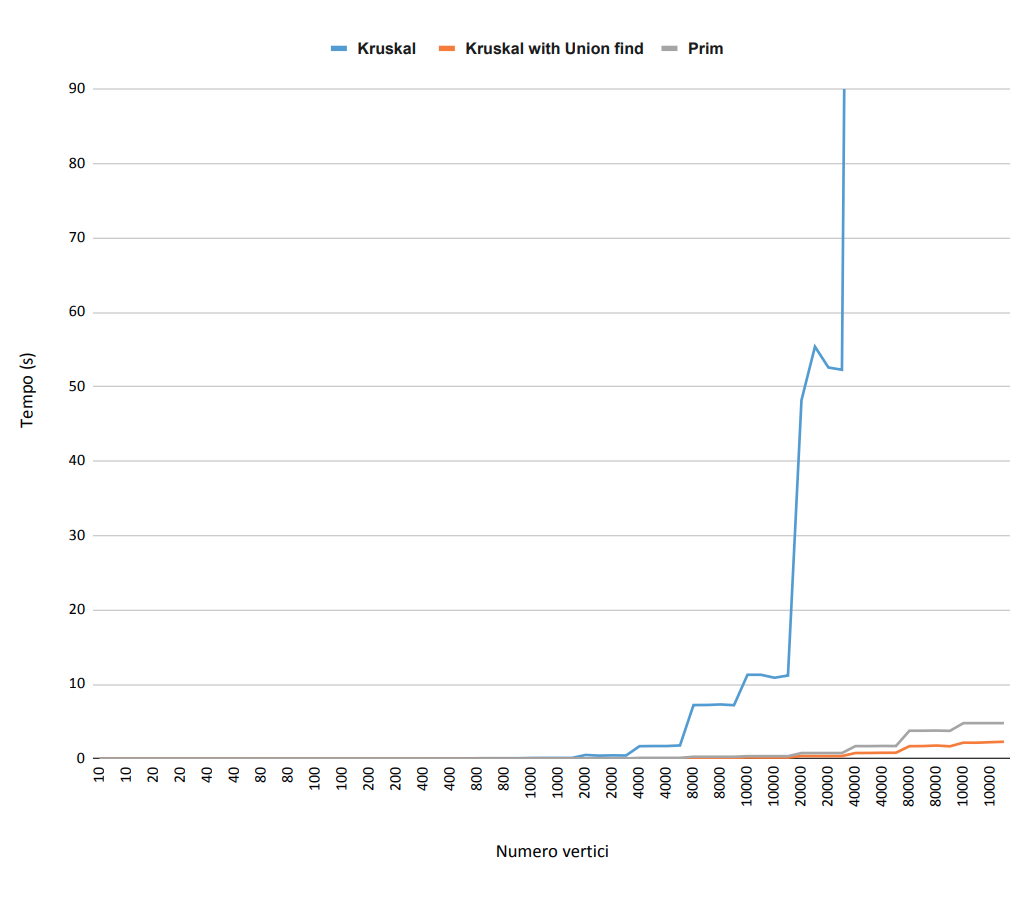
\includegraphics[width=19cm]{Img/compare.png}
	\caption{Confronto tra le performance dei tre algoritmi}
	\label{comparison}
\end{figure}

Dalla Fig.~\ref{comparison} è possibile osservare che per grafi di piccole dimensioni, quindi con un numero di vertici circa pari o inferiore a $1000$, la differenza di prestazioni dei diversi algoritmi non è molto evidente. 
Quando le dimensioni dei grafi di input aumentano, i tempi di esecuzione dell'algoritmo di Kruskal con implementazione ``naive'' crescono in maniera esponenziale fino ad impiegare svariati minuti per effettuare il calcolo del MST per i grafi più grandi presenti nel dataset. 
Gli altri due algoritmi, Prim e Kruskal con Union find, hanno tempi di esecuzione più simili tra loro: pochi secondi per il calcolo del MST anche su grafi di grandi dimensioni. \\
Questi risultati sono coerenti con le complessità degli algoritmi, infatti quello con la complessità più alta è Kruskal in versione ``naive''. 
Gli altri due, invece, presentano la stessa complessità algoritmica sebbene sia possibile affermare che l'algoritmo di Kruskal implementato con Union find presenta dei tempi di esecuzione inferiori rispetto a Prim.

\pagebreak